
\section{MLOps}
\subsection{Project Life-Cycle}
Parliamo della produzione di modelli. Vediamo la pipeline nello specifico dall'immagine seguente:
\\
\begin{figure}[th]
    \centering
    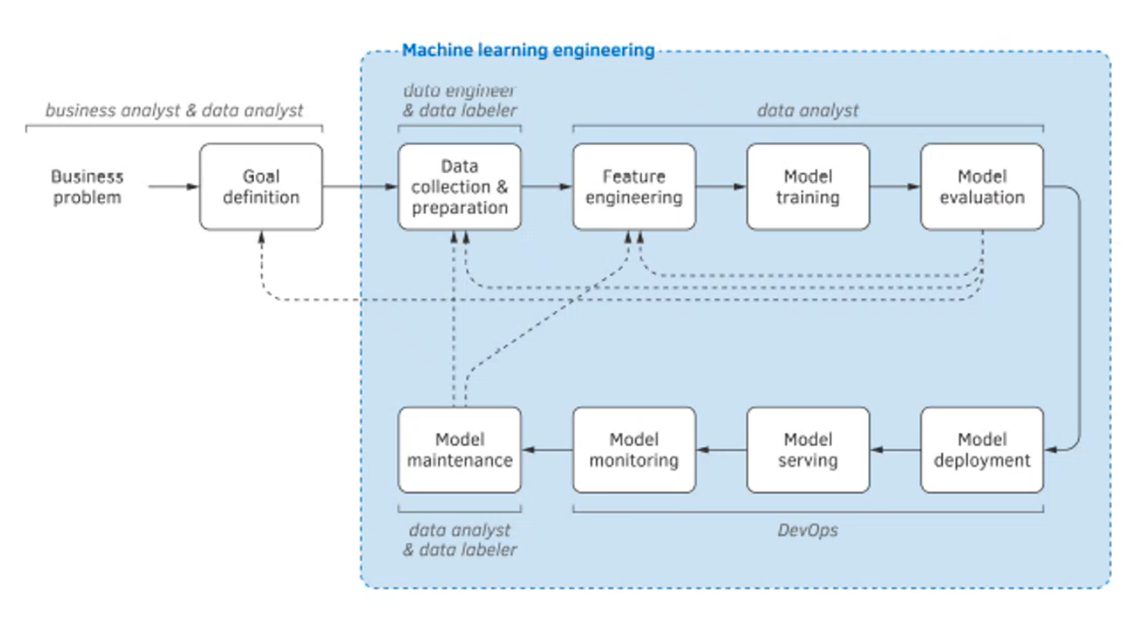
\includegraphics[scale=0.5]{ExplainableAI/img/mlops.png}
\end{figure}
\\
Model deployment, ovvero come viene realizzato (linguaggio); model serving, ovvero come il modello viene utilizzato; model monitoring, il modello va controllato periodicamente. Questo perchè potrebbe non avere le stesse performance che aveva in training e non in produzione. Ci sono diverse regole per cui si può scegliere di usare il ML o si sceglie di non usarlo, dipende molto dalla task, non va usato oltre la necessità. 

\subsection{Perchè i progetti di ML falliscono?}
Le motivazioni principali sono:
\begin{itemize}
    \item mancanza di talento con esperienza
    \item mancanza di supporto dalla leadership
    \item mancanza d'infrastruttura dati
    \item sfida del data labeling: label mancanti vanno aggiunte manualmente
\end{itemize}
In seguito a tutti questi problemi è nata una branca di ML chiamata MLOps che usa delle tecniche per vedere come possa funzionare una tecnica di ML quando viene messa in produzione. 

E ancora: 
\begin{itemize}
    \item quantità di dati: i modelli sono molto sensibili ai dati quindi devono cambiare con loro
    \item decadimento dei modelli: col tempo degrada
    \item località: modelli sbilanciati sulla classe da predire
\end{itemize}

\subsubsection{Mettere un modello in produzione: mlops}
Ovviamente messa in produzione intendiamo rendere il servizio utile al pubblico. Di conseguenza, il modello dovrà avere delle determinate performances, per essere ritenuto all'altezza della produzione. Un modello potrebbe stare in produzione per anni senza alcun guadagno, l'operazione di Ops è necessaria. 
\\
Ci sono 5 aspetti chiave importanti da sapere nei MLOps:
\begin{itemize}
    \item sviluppo
    \item deployment
    \item monitoring
    \item iterazione
    \item governance
\end{itemize}

\subsubsection{Problemi con i dati}
Molto spesso poi ci sono problemi con i dati:
\begin{itemize}
    \item Costi elevati
    \item Scarsa qualità 
    \item Rumore
    \item Bias  
\end{itemize}
Bias è una polarizzazione, il dato pende verso una decisione. Ci sono diversi tipi di bias, ma il concetto è sempre questo: il bias influenza tanto la decisione del modello perchè i dati sono fortemente influenzati. Oppure una classe sbilanciata, che tratto attraverso l'oversampling o l'undersampling: over aggiungo degli elementi in maniera randomica basandosi sugli altri dati (data augmentation). Undersampling fa la stessa cosa ma rimuove delle righe. 
\\
Tutte queste operazioni fanno parte della pipeline del data engineer: data ingestion, dove acquisiamo i dati, exploration e validation, dove si analizzano i dati raccolti, data wrangling, che comprendono tutte le operazioni di pulizia dei dati, data labeling, dare etichette, data splitting dove prepariamo il dataset per il modello. 

\subsubsection{Training and evaluation}
Quando si crea il modello ci sono poi delle fasi da seguire:
\begin{itemize}
    \item Training: tuning degli iperparametri durante la fase di training del modello
    \item Evaluation: allenato sui dati finali per poter essere utile all'utente
    \item Testing: test finale di accettazione 
    \item Model packaging: esportazione del modello in un formato definito
\end{itemize}

\newpage

\subsection{Fairness in ML}
La fairness è importante perchè i dati possono essere una rappresentazione distorta di ciò che è giusto. I modelli imparano le disparità involontariamente, ad esempio la disparità geografica (modelli razzisti). Questo prende il nome di bias preesistente. Esistono altri due tipi di bias, che sono quello tecnico e quello emergente.
\\
Il bias tecnico viene fuori nella fase di prediction con dati non corretti o mancanti, che va ad amplificare spesso e volentieri il bias preesistente. \\
\textit{Esempio.} Persone che mettono il sesso, altre non lo mettono. Il modello guarda la distribuzione che conosce e ipotizza i dati mancanti, ma non è detto che sia il risultato corretto. Un'altra cosa potrebbe essere lo stemming, le parole leaves (foglie) e lasciare (leave) abbreviate sono leav uguali. 
\\
Anche il ranking introduce un errore, il primo sarà un risultato buono ma non sempre è nell'ordine corretto. Infine, l'emergent bias si manifesta come 'ricco che diventa più ricco', vado ad influenzare ad esempio nella raccomandazione di un film e modifico troppo la scelta. 

\subsubsection{No fairness through unawareness}
Rimuovere o ignorare attributi sensibili che possono essere inefficaci e pure dannosi, perchè alcune correlazioni del dataset potrebbero risultare poi troppo deboli. 
\\
A volte le feature sensibili sono ridondanti se ci sono altre feature però se le rimuoviamo il classificatore troverà ridondanza altrove. 

\subsubsection{Pitfalls of action}
Una volta creato il modello si generano le risposte. Si guardano le azioni e i feedback. Ovvero si guarda come agisce e si capisce il feedback del modello. Il feedback può essere interpretato per migliorare il modello come nei search engine. 
\\
Esistono 3 tipologie di feedback:
\begin{itemize}
    \item \textbf{Self fullfilling prediction:} se il modello prevede correttamente, il retraining rafforzerà la predizione fatta
    \item \textbf{Predizioni che influenzano il training set:} il modello predittivo causerà degli arresti, che verranno aggiunti al training set e continueranno ad essere considerate come zone ad alto rischio
    \item \textbf{Predizioni che influenzano fenomeni o la società in larga scala:} il comportamento delle forze dell'ordine, colmo di pregiudizi, influenzerà la povertà e i crimini delle zone a rischio
\end{itemize}

\subsubsection{Statistical non-discrimination criteria}
Questo criterio mira a definire l'assenza di discriminazione attraverso espressioni statistiche, coinvolgendo variabili aleatorie descrivendo lo scenario di classificazione. 
\\
Variabili random (A,R) devono soddisfare l'indipendenza se la predizione che facciamo è indipendente dall'attributo sensibile, quindi A è irrilevante, e tale indipendenza viene chiamata demographic parity. 
\\
\textbf{Il demographic parity basta?} Questo valore è scorrelato dall'accuracy sul dataset perchè è una misura del modello che prevede qualcosa, ma non della sua accuracy. Questa prende anche il nome di Indipendence, ovvero la prediction non è influenzata da feature inutili (es: uomo, donna). 

\subsubsection{Separation}
Lo score di una predizione e l'attributo devono essere indipendenti dalla predizione. Fondamentalmente, tutti i modelli devono fare gli stessi errori in tutti i gruppi della variabile sensibile. 

\subsubsection{Sufficiency}
Le variabili random (R,A,Y) soddisfano la sufficiency se $Y \bot A |R$ che è il simbolo della separation. Se il classificatore prevede 1, quando la probabilità è 0.5, questa deve rimanere 0.5 in tutti i gruppi sociali.
\\
\begin{figure}[th]
    \centering
    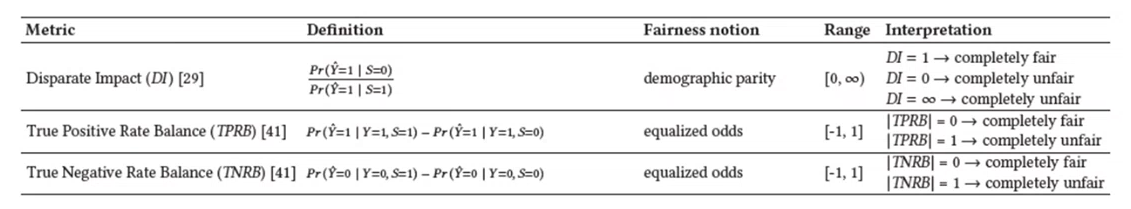
\includegraphics[scale=0.6]{MLOps/img/metriche.png}
\end{figure}

\subsection{Come rimuoviamo gli stereotipi?}
Esistono 3 tecniche per rimuoverli: pre-processing, in-training, post-processing. Differiscono ovviamente per dove sono inseriti. Tra i due quello più sicuro è il preprocessing, ovvero che viene fatto prima della produzione del modello. Quello in-training è sul discorso dei pesi durante il training. 